\documentclass[output=paper,hidelinks]{langscibook}
\ChapterDOI{10.5281/zenodo.13347678}

\title[Languages as public goods]{Languages as public goods and language change as a tragedy of the commons} 
\author{Gerhard Schaden\affiliation{Université de Lille; CNRS UMR 8163 STL}}

\abstract{This paper makes three claims: first, that constructions in languages can be largely analyzed as public goods; second, that in cases where this is not true, they are common pool resources; and third, that in communication, there are systematic and intrinsic conflicts between speaker and hearer, such that in some cases, those conflicts will lead to a tragedy of the commons. 

It will be argued that at least some instances of language change can be seen as cases where short-term speaker interests impose costs on short-term hearer interests, and that in the long run, they also go against the best interests of speakers.}

\IfFileExists{../localcommands.tex}{
  \addbibresource{../localbibliography.bib}
  \usepackage{tabularx,multicol}
\usepackage{url}
\urlstyle{same}

\usepackage{listings}
\lstset{basicstyle=\ttfamily,tabsize=2,breaklines=true}

\usepackage{langsci-optional}
\usepackage{langsci-lgr}
\usepackage{langsci-gb4e}
% \usepackage{langsci-textipa}

\usepackage{csquotes}
\usepackage{multirow}
\usepackage{colortbl}
\usepackage{ulem}
\usepackage{graphicx}
\usepackage{amsmath}
\usepackage{nicefrac}
\usepackage{tabto}
\usepackage{subcaption}
\usepackage{enumitem}
\usepackage{subcaption}


\usepackage{siunitx}
\sisetup{detect-weight=true, detect-family=true, detect-all, input-symbols={\%}, free-standing-units,group-digits=false,detect-inline-weight=math}

\usepackage[linguistics, edges]{forest}
\usetikzlibrary{matrix, arrows, arrows.meta}

\usepackage{pgfplots}
\usepgfplotslibrary{colorbrewer}
\pgfplotsset{cycle list/Dark2-4}

\usepackage{derivative}
\usepackage{langsci-branding}

  
\AtBeginDocument{%
  \SetupAffiliations{output in groups = false, 
                     separator between two = {\bigskip\\},
                     separator between multiple = {\bigskip\\},
                     separator between final two = {\bigskip\\}
                   }%
}

\newfontfamily\cjkfont
  [Scale=MatchLowercase]{SourceHanSerifSC-Regular.otf}
\AdditionalFontImprint{Source Han Serif}

\newcommand{\SC}{S\=uzh\=ou Chinese}
\newcommand{\MC}{Standard Chinese}
\newcommand{\THW}{T\`{a}ih\'{u} W\'{u}}
\newcommand{\SH}{Sh\`{a}ngh\v{a}i}
\newcommand{\iz}{ɨ̻}
\newcommand{\yz}{ʉ̻}
\newcommand{\zz}{ɿ}
\newcommand{\zw}{ʮ}
\newcommand{\pri}{*\textit{i}}
\newcommand{\pry}{*\textit{y}}
\newcommand{\prien}{*\textit{jen}}
\newcommand{\pryen}{*\textit{ɥɤn}}

\newcommand{\spr}[1]{\textsuperscript{#1}}

\renewcommand{\NG}{ŋ}
\newcommand{\textsubarch}{̯}
\renewcommand{\textschwa}{ə}
\renewcommand{\textprimstress}{ˈ}
\renewcommand{\textltailn}{ɲ}

\renewcommand{\textbabygamma}{\textramshorns}
\newcommand{\textramshorns}{ɤ}
\renewcommand{\textbardotlessj}{ɟ}
\renewcommand{\textbari}{ɨ}
\renewcommand{\textbeta}{β}
\renewcommand{\textctc}{ɕ}
\renewcommand{\textdyoghlig}{ʤ}
\newcommand{\textepsilon}{ɛ}
\renewcommand{\textesh}{ʃ}
\renewcommand{\textfishhookr}{ɾ}
\renewcommand{\textglotstop}{ʔ}
\renewcommand{\textlengthmark}{}
\renewcommand{\textopeno}{ɔ}
\newcommand{\textphi}{ɸ}
\renewcommand{\textrevepsilon}{ɜ}
\renewcommand{\textrtailr}{ɽ}
\renewcommand{\textrtailt}{ʈ}
\renewcommand{\textscriptg}{ɡ}
\renewcommand{\textthorn}{þ}
\renewcommand{\textturna}{ɐ}
\renewcommand{\textturnm}{ɯ}
\renewcommand{\textturnv}{ʌ}
\renewcommand{\textyogh}{ʒ}
\renewcommand{\textramshorns}{ɤ}
\renewcommand{\textbabygamma}{\textramshorns} %babygamma obsolete
\renewcommand{\textturnm}{ɯ}

\newcommand{\tone}[1]{\textsuperscript{#1}}
\newcommand{\underarch}{\textsubarch}

\newcommand{\sg}{\textsc{sg}}


\makeatletter
\let\thetitle\@title
\let\theauthor\@author
\makeatother


\newcommand{\togglepaper}[1][0]{
%   \bibliography{../localbibliography}
  \papernote{\scriptsize\normalfont
    \theauthor.
    \titleTemp ~
    To appear in:
    Dankmar W. Enke,   Larry M. Hyman,   Johanna Nichols,   Guido Seiler \&  Thilo Weber
    Language change for the worse.
    Berlin: Language Science Press. [preliminary page numbering]
  }
  \pagenumbering{roman}
  \setcounter{chapter}{#1}
  \addtocounter{chapter}{-1}
}


\newcommand{\ilit}[1]{#1\il{#1}}
  %% hyphenation points for line breaks
%% Normally, automatic hyphenation in LaTeX is very good
%% If a word is mis-hyphenated, add it to this file
%%
%% add information to TeX file before \begin{document} with:
%% %% hyphenation points for line breaks
%% Normally, automatic hyphenation in LaTeX is very good
%% If a word is mis-hyphenated, add it to this file
%%
%% add information to TeX file before \begin{document} with:
%% %% hyphenation points for line breaks
%% Normally, automatic hyphenation in LaTeX is very good
%% If a word is mis-hyphenated, add it to this file
%%
%% add information to TeX file before \begin{document} with:
%% \include{localhyphenation}
\hyphenation{
affri-ca-te
affri-ca-tes 
Scha-den
Zú-ñi-ga
Kaj-kwa-khrat-txi
}

\hyphenation{
affri-ca-te
affri-ca-tes 
Scha-den
Zú-ñi-ga
Kaj-kwa-khrat-txi
}

\hyphenation{
affri-ca-te
affri-ca-tes 
Scha-den
Zú-ñi-ga
Kaj-kwa-khrat-txi
}

  \togglepaper[12]%%chapternumber
}{}





\begin{document}
\SetupAffiliations{output in groups = true, mark style=alphabetic}
\let\PRES\PRS
\maketitle

\section{Introduction: Public vs private goods}

\citet{samuelson54} introduced an important conceptual distinction by separating two types of goods: private goods vs public goods. Public goods have two essential properties distinguishing them from private goods: if one person uses or consumes a public good, this does not diminish the possibility of consumption by other people (which is called the property of ``nonrivalness of consumption'', or ``subtractability''); the second property is that it is either difficult, prohibitively costly, or outright impossible to exclude other people from using them (which is called ``exclusion''). This has lead economists to further refine this distinction into the four-way classification of goods as illustrated in \tabref{tab:goods},\footnote{A brief note to \tabref{tab:goods}: In the age of high-speed internet, (permanently networked) personal computers are probably not as excludable as they used to be, or as we would like them to be, since knowledgeable hackers can access your device without your knowledge.} where we will focus for the moment on the opposition between public and private goods.

\begin{table}
\caption{4 types of goods, following \citet[9]{hessostrom07a}\label{tab:goods}}
\begin{tabular}{lll}
  \lsptoprule
  Exclusion & \multicolumn{2}{c}{Subtractability}\\\cmidrule(lr){2-3}
            & Low  & High\\\midrule
            &  \textit{Public goods} & \textit{Common-pool resources}\\
  Difficult &  Useful knowledge      &   Libraries\\
            &  Sunsets               &  Irrigation systems\\\midrule
            & \textit{Toll or club goods} & \textit{Private goods}\\
  Easy      & Journal subscriptions   & Personal computers\\
            & Day-care centers        & Doughnuts\\
  \lspbottomrule
\end{tabular}
\end{table}

A prototypical private good -- like a popsicle -- is subtractable and excludable. If I eat the popsicle, this prevents anybody else from eating it. And in most circumstances, it is not prohibitively costly to exclude other people from eating it (either because I eat it, or because I store it in an inaccessible place).

\subsection{Languages as (collections of) public goods}
\label{sec:lang-as-coll}


It appears at first sight that all ingredients of natural languages are public goods.\footnote{As we will see below in \sectref{sec:govern-ling-comm}, certain linguistic expressions do seem to be common pool resources rather than public goods. I will come back to the issue of subtractability in \sectref{sec:some-ling-reso} below.} Clearly, if I use a phoneme (like /s/), this does not prevent other language users from producing it as well. And there is no way for me to monopolize the use of a phoneme. The same thing is true for other linguistic expressions: words, morphemes, constituents, propositions. Languages are basically huge collections of public goods, and their  usefulness derives from the fact that they are public goods. Language, as a conventional signaling system, has by definition no place for completely private signs or phonemes.

Languages (and language units) are not the only public goods. Similar cases include software, audio- and video-files etc. If I use some program or file, it can be copied without problem, and given to other people, without diminishing in any way my personal use. This fact has given rise to all kinds of copy-left licenses. However, it is also a source of problems: given the costs of producing software, music or films, and the ease with which their use can be transferred without diminishing the use of the transferrer, there is no reason why a selfish agent would pay for it. But if nobody pays for such content anymore, this creates a problem for the creators of such content, who cannot afford to create new content anymore. Therefore, given rational agents, the content is predicted to disappear in the long run. This problem is known as the ``tragedy of the commons'' \citep[see][]{Hardin1243}. What I will try to show in this paper is that -- given that units of languages are public goods -- they are probably not immune to such tragedies, and that at least some instances of language change can be classified in this way.

As far as I am aware, there has not been much investigation into the idea that change within one language might be an instance of a tragedy of the commons,\footnote{But see \citet{nikitina18}, although the tragedy of the commons is treated from a very different perspective.} although there is literature in language preservation, dealing with the transition of a community from one language to another.\footnote{This has been pointed out to me by one of the anonymous reviewers; see, e.g., \citet{beckerman96,eggington10}.}  So, the question is: would we expect something like this to happen in language? And whatever the answer may be to this question, why?
As far as I can see, the field of linguistics is stacked against such a position, because it seems to suggest that somehow, a language would have decayed from an anterior, better state. Furthermore, it seems to contradict the idea that all languages can satisfy the same expressive needs. Finally, mainstream pragmatic theories \citep[witness, e.g.][]{clark96} stress collaboration following an interpretation of \citet{grice75}, which is antithetical to the idea of change as deterioration driven by short-term, selfish instincts.

There are also important empirical reasons that one can adduce: as far as I am aware, there has been no catastrophic breakdown of a signaling system -- contrary to attested breakdowns of physical resources --, and I certainly would not expect that speakers discard a language for having become too unwieldly to be spoken, and adopt another one. Finally, languages (like other memeplexes, see \citealt{blackmore99}) seem to lack the crucial property of subtractability that physical resources have: they cannot be exhausted, and contrary to other cultural resources, there is no special creativity involved in creating utterances.\footnote{I am speaking here of the kind of creativity that one might be willing to reward with a protection by copyright, like our societies have decided to do for patents, works of art, or software. I assume that even in our age of patent- and copyright-trolls, nobody would seriously consider a protection for a specific grammatical construction, such that McDonald's would obtain a copyright on the progressive, or Nike on \emph{do}-support in \ili{English}.} Thus, there are good reasons to doubt that a tragedy of the commons could be an issue for a linguistic resource. 

In the remainder of this introduction, I will show why the tragedy of the commons is of importance to linguistics. I will start by considering what kind of conditions stabilize systems against tragedies of the commons. Then, I will show that at least some linguistic expressions are indeed subtractable. Finally, I will go on to show how even linguistic entities that are not subtractable may still be susceptible to selfish exploitation by speakers.

\subsection{Governing the linguistic commons}\largerpage
\label{sec:govern-ling-comm}

The tragedy of the commons is notable for the fact that rational behavior (as defined in the usual, game-theoretic way) leads to bad outcomes for all. In many instances, indeed, such bad outcomes have come to pass (e.g., global warming, pollution, deforestation, or the collapse of fisheries). However, there all also many instances of commons that have been managed in a sustainable way, and therefore, avoided to turn into tragedies. \citet{ostrom90} has studied cases of successful vs unsuccessful cases of making common pool resources use sustainable. \citet[90--102]{ostrom90} identified the following ``design principles'' for long-enduring institutions able to successfully govern common pool resources (for material goods):\footnote{The shortened formulation of these design principles is taken from \citet[7]{hessostrom07a}.}

\begin{itemize}
  \item Clearly defined boundaries should be in place;
  \item Rules in use are well matched to local needs and conditions; 
  \item Individuals affected by these rules can usually participate in modifying the rules;
  \item The right of community members to devise their own rules is respected by external authorities;
  \item A system for self-monitoring members' behavior has been established;
  \item A graduated system of sanctions is available;
  \item Community members have access to low-cost conflict-resolution mechanisms;
  \item Nested enterprises -- that is, appropriation, provision, monitoring and sanctioning, conflict resolution, and other governance activities -- are organized in a nested structure with multiple layers of activities
\end{itemize}

The question is whether these principles do apply at all to language (or linguistic constructions). At first sight, the answer seems to be negative. First of all, monitoring language is not that easy, since many people seem hardly to be aware of a large part of their linguistic production. There is also no low-cost conflict-resolution mechanism in place for the ``correct'' use of a linguistic resource -- and probably, there is no way of deciding on the ``correct'' way of use of a linguistic  resource (or more generally, a resource based on convention) at all. In any case, language academies (where they do exist) do not seem to be able to fulfill such a role. Furthermore, it is not that clear in all instances (even for trained linguists) where the exact boundary of a linguistic construction should be drawn. Finally, and most importantly, these design principles have been observed for common pool resources, and not public goods. As discussed above, the difference of these two kind of resources is subtractability: a public good is not subtractable (and the use of one person does not impede other persons from using them). However, the fact that something is non subtractable does not guarantee immunity against tragedies of the commons, as was illustrated by (media or software) piracy. I will come back to this issue in \sectref{sec:trag-comm-with}. However, as will be seen in \sectref{sec:some-ling-reso}, at least some linguistic items are subtractable.

If we ignore for a moment the narrower issue of linguistic expressions as public goods vs common pool resources, Ostrom's criteria also give us an idea in which cases linguistic commons cannot be enforced (or only with much difficulty). First, the observance of some convention can only be enforced if its non-observance can easily be detected. Second, if there are no sanctions, or if access to sanctions is prohibitively costly, even detection will be of no use. Third, if encroachment or appropriation of the commons is not resisted by insiders of the group defending some particular use, there also will be little chance of resisting a use. In the case studies presented in \sectref{sec:two-case-studies}, difficulty of detection will be the most salient point. However, the difficulty or resistance towards outsiders will be of importance what follows in \sectref{sec:some-ling-reso}.


\subsection{Subtractable linguistic entities}
\label{sec:some-ling-reso}

The use of commons does not happen in a void; in our intensely social species, it always happens within social groups. Therefore, it is worth stressing that the use of commons is always defined by \citet{ostrom90} as the use of some resource \emph{by some community} -- and this social aspect may introduce subtractability.

A linguistic resource (like a word) may be used by other speech communities (i.e., speakers of other languages), but at first sight, this does not seem to be problematic: because of the absence of subtractability, loans need not have any impact on the source language. For instance, it is a source of amusement to \ili{French} native speakers that in \ili{German}, hairdressers are called \emph{Frisör} (which is a loan from \ili{French}, and means literally `one who makes locks'), but this does not subtract anything from the possibility of using \emph{friseur} or \emph{coiffeur} (which is the normal \ili{French} correspondent of \textit{hairdresser}) in \ili{French}. Generally, the fact that speakers of some language $A$ take some lexical element from some language $B$ does not seem to interfere with usage in language $B$. Speakers of different languages do not interact frequently enough (in the general case, and in their respective mother tongues) for such a loan to have any perceivable effect on the source language. In order to see cases where a linguistic commons is defended as the exclusive property of one community (and sensibly so), we probably need to look at linguistic resources specific (or defended as being specific) to socio-linguistic communities within a larger language community.


The basic issue is that, while it is most often true that the use of a linguistic expression by some person cannot prevent its use by some other person, the use of a linguistic expression by some persons in \emph{some specific sense} can nevertheless impact its use \emph{in some (possibly different) sense} by other persons, and may influence that usage to a degree that speakers of one group no longer see it fit to serve its purpose. Let us take a (fictive) example to illustrate this behavior: assume that linguists somehow come to acquire a word for everything that is linguistically cool, namely ``ʃwɛt'', and that this word is commonly used in \ili{English} conversation among linguists, and also, in online discussion, for instance on LanguageLog. Things that are ʃwɛt are ergative languages, Burushaski, retroflex consonants, quirky voice, etc. Now assume that Justin Bieber, a regular reader of LanguageLog, starts to use ʃwɛt in his tweets, and that his fan-base starts using this expression to qualify things that appear cool to them (certainly Justin Bieber himself, but also the lyrics of Justin Bieber songs, Justin Bieber posters, etc.). Since there are more Justin Bieber fans than linguists, there would be no way that ʃwɛt could retain its association with linguistics\footnote{And also, its association in linguists' minds with more futile concepts like cultural sophistication, excellent taste, etc.} in the larger population, and the use of ʃwɛt would mark its utterer as a fan of Justin Bieber -- with all its associations. Most likely, linguists would end up abandoning its use. In this context, ʃwɛt could function as a badge for membership in a small community as long as its use was -- in the mind of the members of that community -- strongly associated with group membership. So, especially if an expression is used to encode group membership or social distinction or differentiation, one of its main appeals may be the fact that it is not used by salient out-group members.\footnote{This is not specific to linguistic expressions; the same is true for other cultural artifacts, as can often be seen in the commercialization of (formerly ``underground'') sub-cultures.} 

%A real-life example of such the abandonment of a word due to an external shock comes from \ili{German} (even though the phenomenon is reflected also in other languages), and concerns linguistics (among others). In the second half of the 19\textsuperscript{th} and the beginning of the 20\textsuperscript{th} century, the term \emph{Aryan} (\ili{German} \emph{arisch} as an adjective) \emph{could} be used as a technical term in linguistics,\footnote{It is possible that the use of \emph{arisch} as opposed to \emph{indogermanisch} always came with a hint of social meaning of sympathy with movements that we would qualify today as extreme right-wing. Thus, the shift in associative meaning may not be as complete as in the fictive example above. However, the fact remains that this term can be found in grammars as a technical term simply meaning \ili{Indo-European}, see, e.g., Max Müller's \emph{Vorlesungen über die Wissenschaft der Sprache}, \href{http://mdz-nbn-resolving.de/urn:nbn:de:bvb:12-bsb11104518-2 }{http://mdz-nbn-resolving.de/urn:nbn:de:bvb:12-bsb11104518-2}, dating from 1866.} referring to either \ili{Indo-European} or \ili{Indo-Iranian}. Nowadays, this word has been completely replaced by \emph{indogermanisch}.\footnote{It still subsists as part of a compound word in \emph{indoarisch}, to refer to the \ili{Indo-European} languages of India.} The reason of this disappearance is probably not only its ambiguity, or an alignment with international scientific practice, but also its strong association with (\ili{German}) right-wing ideology and racism (beginning already in the 19\textsuperscript{th} century). The final nail in the coffin came from its use by the Nazi party. To any \ili{German} speaker living today and who is not a neo-Nazi, the term \emph{arisch} has been tainted beyond recovery. Figure \ref{fig:aryan}, from Google's n-gram viewer, displays frequencies of the term ``\ili{Aryan}'' in collocations which are (at least potentially) scientific terms. As can be seen, the dominance of the term in potentially technical uses dates principally from the end of the 19\textsuperscript{th} century, but there is also a spike around 1940, which corresponds to the time of the third Reich. 
%
%\begin{figure}
%  \centering
%  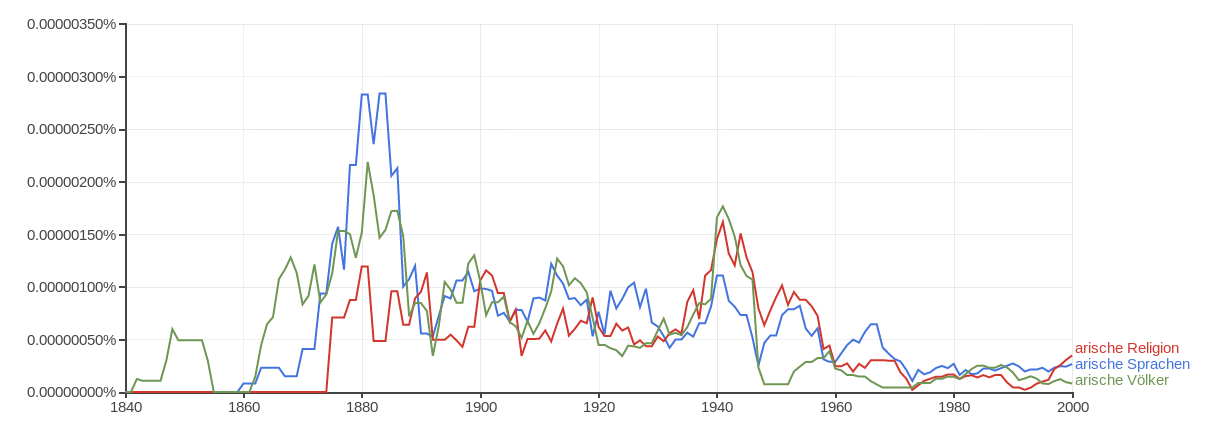
\includegraphics[width=1.0\textwidth]{figures/arian-google-ngram-cropped}
%  \caption{Time-line of \emph{arisch} in (potentially technical) collocations in German books. Source: Google N-Gram Viewer (\href{https://books.google.com/ngrams}{https://books.google.com/ngrams})}
%  \label{fig:aryan}
%\end{figure}
%
%If we contrast these technical uses with the global use of the term \emph{Aryan} as depicted in \figref{fig:aryan-general}, one can see that here, the spike in use during the third Reich was much more pronounced -- which is not very surprising, given the Nazi's preoccupation with race. But there was no way in which a small linguistic subfield could have protected the term against its association with Nazi ideology, which lead in the end to its abandonment as a neutral, technical term.
%
%\begin{figure}
%  \centering
%  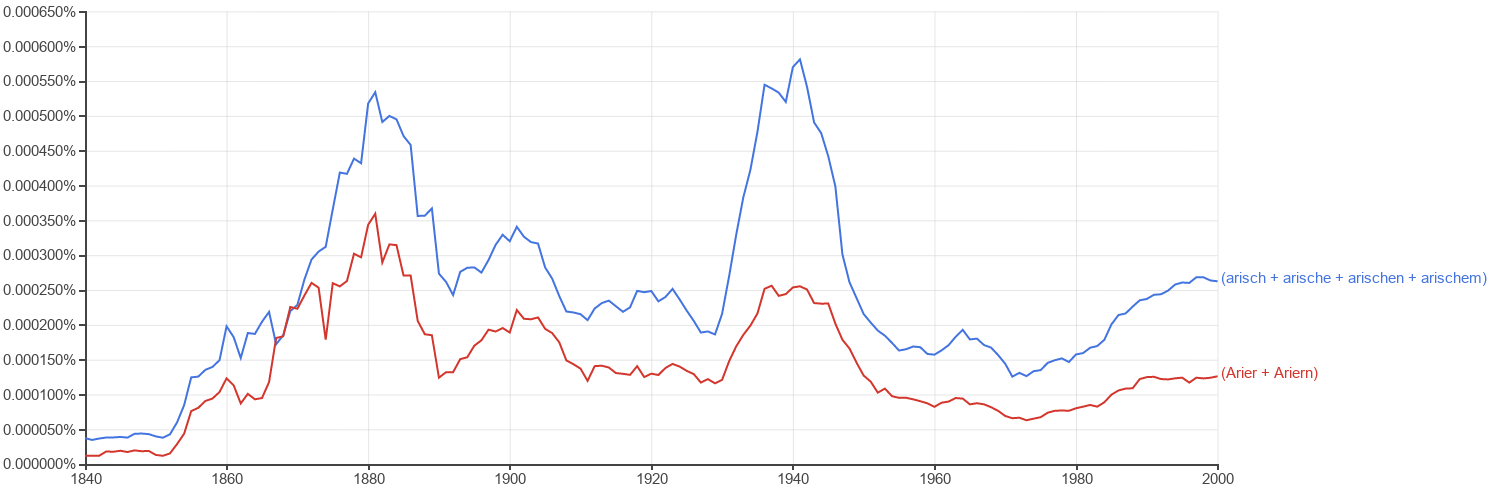
\includegraphics[width=1.0\textwidth]{figures/google-arisch-cropped1}
%  \caption{Time-line of \emph{arisch} and \emph{Arier} in German books. Source: Google N-Gram Viewer (\href{https://books.google.com/ngrams}{https://books.google.com/ngrams})}
%  \label{fig:aryan-general}
%\end{figure}

Now, are there any cases of the successful defense of a positively connoted meaning of a word by some group in the face of out-group adversity? One possible case
comes from the N-word. As cursory listening to Afro-American rap artists will show, it is highly frequent in some socio-linguistic communities of Afro-Americans in the United States, and does not have any derogatory meaning attached \emph{in that specific context}. At the same time, it is also used by white supremacists, in which case it has a strongly derogatory meaning, and is also historically tainted by its  use by slave-owners. As of the writing of this paper, the use of the N-word by others than African-Americans is completely beyond the pale in polite company, and even its mention (in citations, with scare-quotes) has become taboo.

To what extent can this be seen as a successful defense of a commons? It concerns the use of a linguistic resource (a word), whose use is polluted by at least a part of the out-group (i.e., white supremacists). Nowadays, the wish of the Afro-American community not to be addressed at or referred to in this demeaning way is respected by external authorities (not all, but the taboo on the N-word has a wide political, social and media backing). There is a graduated system of sanctions, reaching from a slap on the wrist on social media or booing in a concert for \ili{Caucasian} students singing rap songs containing the N-word, to the temporary or permanent loss of political functions or jobs.\footnote{For the smaller sanctions, see \url{http://theconversation.com/white-people-should-never-rap-the-n-word-a-linguist-breaks-it-down-84673}, retrieved on 26/05/2018; for an instance of the latter, see, e.g., \url{https://en.wikipedia.org/wiki/Anne_Marie_Morris}, retrieved on 25/05/2018, or \url{https://www.theroot.com/new-york-times-hires-fires-reporter-for-using-the-n-wo-1822995189}, retrieved on 6/6/2018. What is interesting about these cases is that it is not that clear that overt racism was the driving force behind the utterance of the N-word.}
Social media provide for a low-cost means of gaining redress; social shunning or exclusion can work on multiple levels (family and friends, work, etc.), and the use of a word is something that can be easily monitored and documented.

What I take these examples to show is that the use of a linguistic form with some meaning by one group can have an impact on the use of that same linguistic form (but with a possibly different meaning) by some other group. Therefore, at least some linguistic expressions are subtractable, and thus, common pool resources rather than public goods. And while the linguistic commons can sometimes be successfully defended, there are also cases where the association with an unsavory group leads to an abandonment of the resource.

\subsection{Tragedies of the commons with non-subtractable public goods}
\label{sec:trag-comm-with}

The main point I will defend in the remainder of the article is that some instances of grammatical change can be seen as tragedies of the commons. This does not seem obvious at first, because grammatical items (like articles, tense morphemes, etc.) do not seem to be subtractable. However, as already explained in \sectref{sec:lang-as-coll} above, tragedies of the commons are not necessarily limited to common pool resources, and can also concern public goods, like (records of) music, or (electronic) texts, or useful knowledge more in general.

The argument in cases of knowledge commons generally concerns the production aspect. Writing a novel takes a lot of time and effort, and an author (or musician) should ideally earn some money with it. If there is no reward for the effort (because sales are preempted by massive free online copying), a rational agent should not engage in the creation of novels (or music). Therefore, we would end up with no new art. Similarly, if anybody could freely sell any new medical molecule or processor design, rational corporations would stop doing research and development, and we would end up without new drugs and faster computers. The net effect would be the end of innovation, and therefore, stagnating culture.

The question is whether this could concern linguistic entities. At first sight, the obvious answer seems to be negative. As far as I know, nobody is doing research on the structures of \ili{English}, with the aim that speakers of that language could tell their husband or wife in 40\% less time what they have been doing during the day, in order to free them for more productive tasks. So, in that sense, there is no innovation that could be stifled. However, I will argue in \sectref{sec:confl-betw-speak} that tragedies of the commons in linguistics are linked to production, although in a slightly different way.

The remainder of this paper is structured as follows: in \sectref{sec:confl-betw-speak}, I will lay out the basic hypothesis, namely that speakers and hearers have opposing preferences in communication, and that these may be the origin of a tragedy of the commons. In \sectref{sec:two-case-studies}, I will look at two different diachronic changes that illustrate these opposing preferences in action, and how in the long run, these lead to less favorable outcomes for everybody. \sectref{sec:concl-persp} concludes the paper.


\section{The conflicting interests of speakers and hearers in communication}
\label{sec:confl-betw-speak}


The two main points the remainder of this paper will try to make are the following: first, there are factors where selfish instincts of the speaker will lead to a situation that is worse for the hearer, and that, as a consequence, this can lead in the long run to a situation that is worse for the speaker, as well; and second, that a rational speaker has an incentive to transfer communication costs toward the hearer. 

\subsection{Motivating the idea}
\label{sec:motivating-idea}

The idea of an intrinsic conflict between speaker and hearer in communication may be highly counterintuitive. An objection can be stated as follows: Aren't we all speakers and hearers all the time? Why should we do as speakers something that would hurt us as hearers? This would obviously be stupid, so why would anybody do this? If this argument looks convincing to you, consider the following, which has \emph{exactly} the same structure. Aren't we all tax payers and do we not all receive the benefits of our taxes (infrastructure, etc.)? Why would we do anything as tax payers that would hurt us as the receivers of benefits? Clearly, evading taxes would be extremely stupid, and we should not expect anybody to engage in such an obviously hare-brained endeavor.

Now, we know that some people do engage in evading taxes, and tax fraud is a problem in many, if not all, countries. The point to be made here is not only that incentives may vary (some people receive vastly more money than they pay, and vice-versa); even if someone pays very little, and receives huge amounts, there would still be an incentive not to pay taxes at all. So, individually, evading taxes does make sense -- and if only one person does it, the consequences on a country's budget will be so small as to be negligible. The problem, of course, is that everybody has an incentive to evade taxes, and if nobody pays taxes anymore, there will be no benefits to be distributed. In what follows, I will argue that exactly the same pattern as in tax fraud -- an incentive for an individual, which is detrimental for the collective, and in the end, also the individual -- also holds in linguistic communication. The literature on evolutionary biology assumes that biological organisms are designed by evolution to be utility-maximizers -- an assumption even shared by authors working explicitly on the evolution of altruism \citep[see, e.g.,][]{bourke11} --  and I will assume that this behavior is too deeply engrained not to be operative in language use.

So, what are the conflicting interests of a speaker and a hearer? Communication involves a hearer figuring out what a speaker had in mind by sending a given message, and it is a process which involves costs for both speaker and hearer. Let us spell this out in a preliminary fashion in (\ref{ex:content}). The information transmitted by a speech act can be taken to the explicitly coded meaning, plus any additional elements inferred by a hearer. In any case, a speaker can assume -- and will depend on the fact -- that the hearer will infer at least some additional content. Explicit coding is associated with costs for the speaker, whereas inference is associated with costs for the hearer. All things being equal, a rational speaker should therefore prefer inference to coding, whereas a rational hearer should prefer coding to inference.%\footnote{In order to get the intuition across more clearly, imagine a high-stake context where a speaker}

\ea \label{ex:content}
cost of communication = cost of coding + cost of inference\footnote{This formulation assumes that the proper act of decoding has a negligible cost with respect to additional inference costs that go beyond pure linguistic decoding. In order to illustrate the difference, consider the following: upon hearing \emph{the president has small hands}, the hearer has to decode that there exists in the utterance context a unique individual who is president, and who has small hands. This, however, is not sufficient to derive truth-conditions for the sentence, since the hearer has to figure out with additional inferences which individual the speaker was referring to by saying ``the president'' in this particular context.}
\z

In extreme cases -- and everything else being equal -- the speaker would prefer not to have to speak at all, whereas the hearer would prefer to rely on inference as little as possible. In order to make things a little less abstract, let me give an example. Assume that a speaker wants to communicate (\ref{ex:drunk}a), and to do so, chooses (\ref{ex:drunk}b), rather than (\ref{ex:drunk}c--d). 

\begin{exe}
  \ex \label{ex:drunk}
  \begin{xlist}
    \ex $\exists x [\text{man}(x) \land \text{see}(m,x) \land \text{drunk}(x) \land \text{can\_hardly\_walk}(x)]$
    \ex Michael saw a man. He was drunk, and could hardly walk.
    \ex Michael saw a man who was drunk and who could hardly walk.
    \ex Michael saw a man. That man was drunk, and could hardly walk.
  \end{xlist}
\end{exe}

(\ref{ex:drunk}b) is a perfectly legitimate -- and probably common -- way of expressing the content of (\ref{ex:drunk}a), and it is likely to have communicative success.
Notice, however, that (\ref{ex:drunk}b) is underspecified with respect to a crucial part of information that is specified in the other alternatives: the identity of the drunk person who could hardly walk anymore. As (\ref{ex:drunk}b) stands, it might be \emph{Michael} or \emph{a man}. At the same time, (\ref{ex:drunk}b) is slightly less complicated to code than (\ref{ex:drunk}c--d) -- it is shorter, and has no subordinate clauses. By using the third-person pronoun \emph{he} in such a context, a speaker leaves a piece of information that could be explicitely coded to be inferred by the hearer. Therefore, the speaker transfers effort to the hearer.

I would like to stress that what I have been exposing here is not a new idea, although as far as I know, the specifics are new. There is a common -- and, as far as I know, well accepted idea -- that language is shaped (among others) by two conflicting forces: \emph{economy} vs \emph{clarity}, on the background of social \emph{conformity} \citep[see, e.g.,][]{keller94,Haspelmath1999optimality}, or already \citep[313ff.]{prinzipien}. The twist I would like to suggest is that these are conflicting interests of a speaker (\emph{economy}) and a hearer (\emph{clarity}) when playing a signaling game (and hence, \emph{conformity}).

Let me rehearse again why individually, it makes sense for a speaker to reduce the coding effort.

\subsection{Modeling the optimization problem}
\label{sec:optimization-problem}

An act of communication is generally modeled as a signaling game. In a signaling game, the speaker observes some state $s$, to which the hearer has no access. Given this state, the speaker then chooses a signal, which he transmits to the hearer (in other words: the speaker strategy maps a state to a signal). The hearer receives the signal, and based on this, must chose some action $a$. If the chosen action is appropriate given $s$, both hearer and speaker receive some payoff; if $a$ is inappropriate given $s$, both receive nothing. Generally, signaling games are treated as being cost-free. But we are interested in the specific case of costs associated with communication, and ignore the coordination part (apart from the effort required).\footnote{Communication cost and how to share it is important also in domains slightly removed from natural language. For instance, the internet has moved from a state where most rendering was done on the server-side to a position where much rendering is done on the client-side (that is, by JavaScript in a web-browser).}

The optimization problem can be stated as follows. For the speaker $S$, it involves choosing a level of effort $γ \geq ε_S$ such that $γ + δ \geq t$ (where $ε_S$ represents the minimally necessary effort on the speaker, $δ$ is the level of effort chosen by the Hearer $H$, and $t$ is the threshold below which communication fails, and above which it will succeed). Similarly, the optimization problem for $H$ can be stated as choosing $δ \geq ε_H$ such that $γ + δ \geq t$. I assume that both $ε_S$ and $ε_H$ need to be positive and greater than 0. The idea is that when a hearer does not pay attention, communication will fail no matter what the speaker may do; similarly, I assume that if the speaker does not make an effort to emit some message, we have left the proper domain of signaling games. As a corollary, this also means that $γ < t$ and $δ < t$.

We can now define the pay-off functions of the two participants:

\begin{exe}
  \ex \label{ex:payoff-func}
  \begin{xlist}
  \ex $p_S(u, γ, δ) = \text{benefit}(u) - \text{cost}(γ)$
  \ex $p_H(u, γ, δ) = \text{benefit}(u) - \text{cost}(δ)$
  \end{xlist}
\end{exe}

(\ref{ex:payoff-func}) assumes thus that the benefit of an utterance is the same for speaker and hearer, but that they may incur differing costs, which has to be subtracted from the (possible) benefit they receive from successful communication. 

\begin{figure}
  \hfill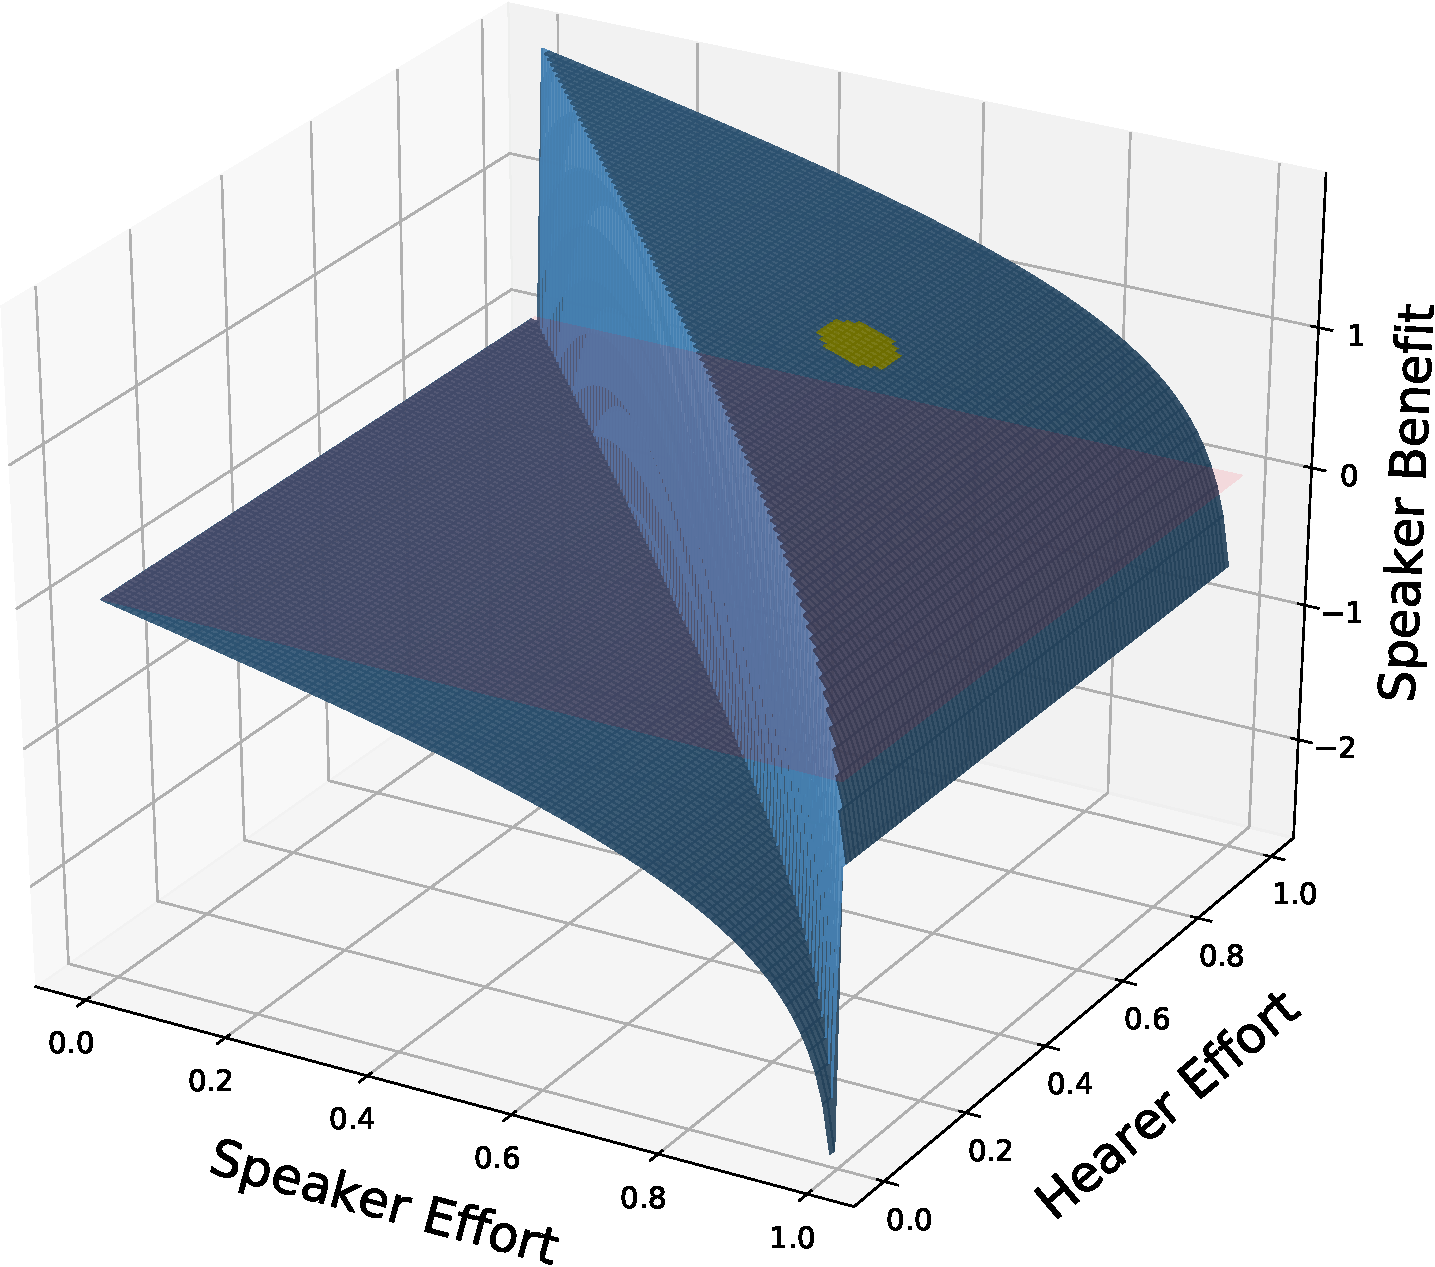
\includegraphics[width=.45\textwidth]{figures/speakerUtility-with-standard-cropped}\hfill%
  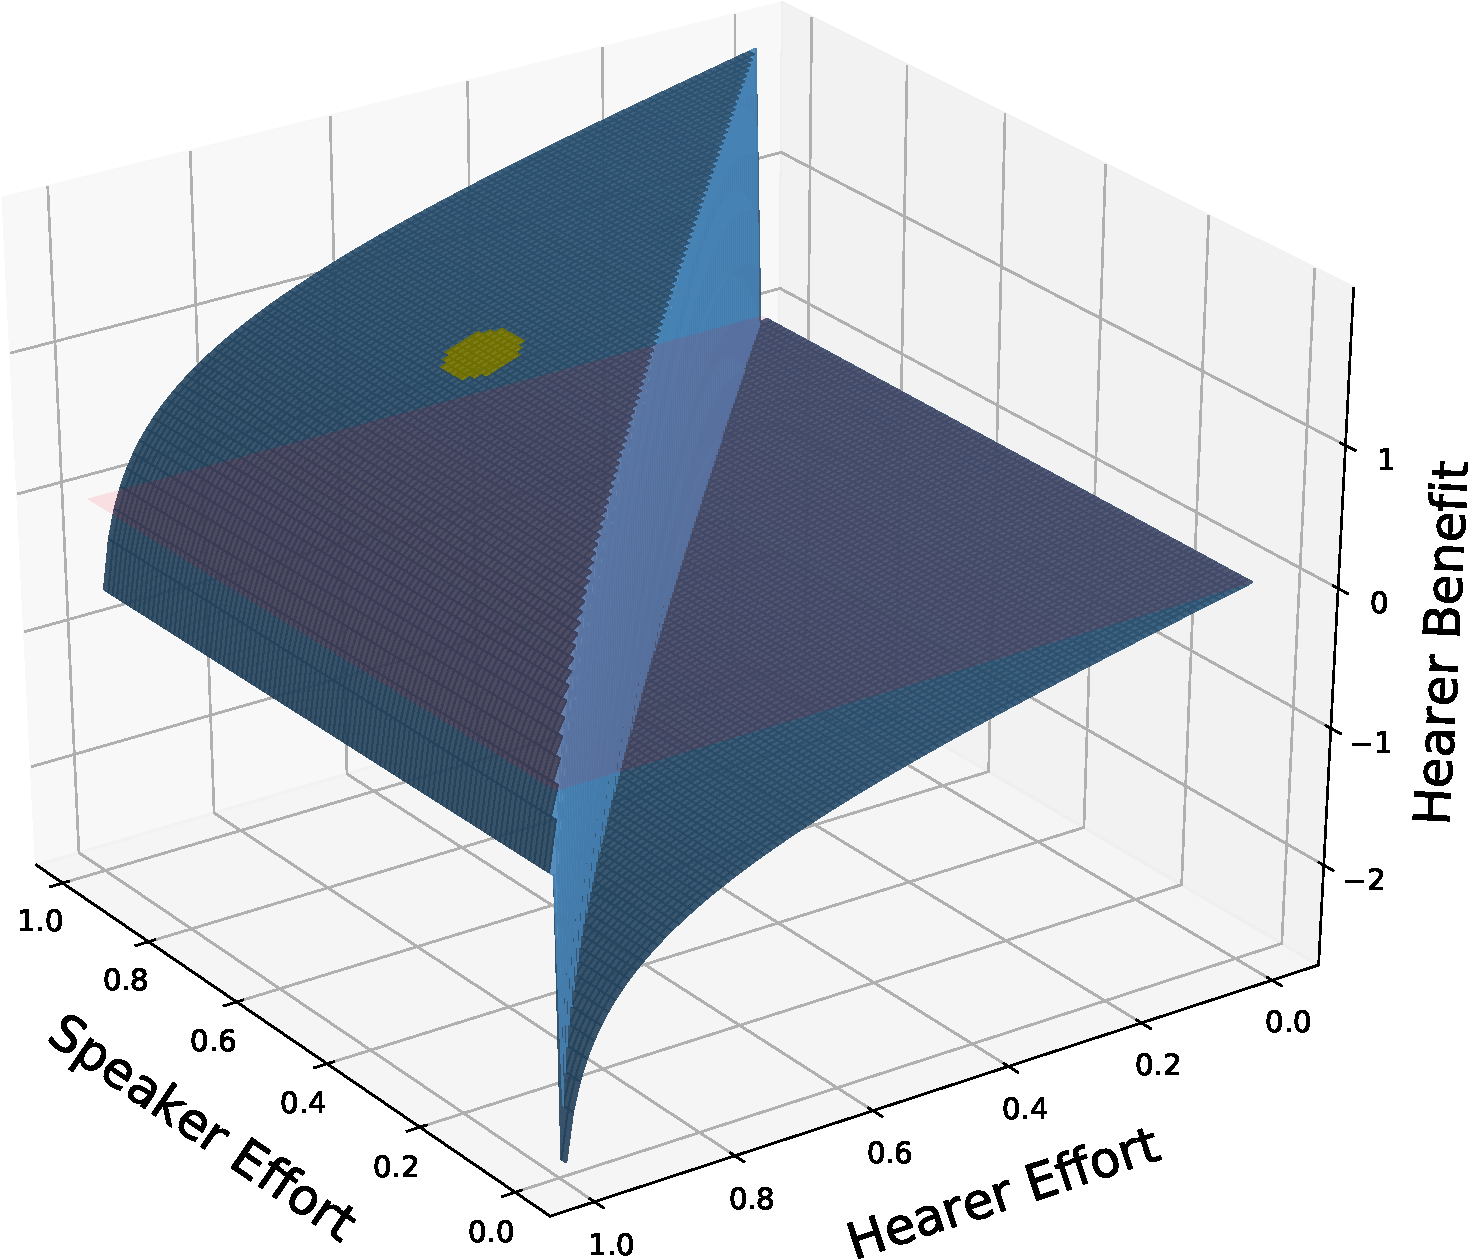
\includegraphics[width=.45\textwidth]{figures/hearerUtility-with-standard-cropped}\hfill%
  \caption{Profiles of speaker (left) and hearer (right) benefits. In yellow: area of socially expected levels of effort in coding and inference.}
  \label{fig:shbenefits}
\end{figure}

As can be easily seen in \figref{fig:shbenefits}, the payoff for each participant is maximized for the lowest admissible level of effort possible, and decreases as the level of effort rises.
In both cases in \figref{fig:shbenefits}, the diagrams show a sharp cliff where successful message transmission borders on non-successful passing of the message. But even when the message is successfully transmitted, the cost may become so high that it would have been better not to attempt to transmit the message. As has often been noted, natural language is a communication system characterized by a high degree of redundancy. One way of conceiving of this is to assume that there is a (social) norm which keeps away a message from the cliff, and that there is something like an expected level of coding (and inference) in the population -- which has been pictured in \figref{fig:shbenefits} by the yellow area.

We can assume that there are sanctions for speakers not conforming to the socially expected level of coding effort. However, this area should probably not be conceived of as a single point that could be easily targeted, but has to cover some acceptable variation. And within this acceptable range of variation, we should expect a rational speaker to minimize effort. Once again, if there is a single speaker doing this within a sufficiently large population, one would not expect this to have any consequences. However, the incentives exist for all speakers, and if all speakers start to minimize their effort, and if the socially expected level of effort is dependent on production at least to some degree, over time, the socially expected area of coding will approach the cliff, and eventually, go over it. Once this has happened, the coding strategy is no longer viable, and has to be replaced.




But let us now look at two concrete cases where rational incentives for the speaker either to minimize coding or to increase the inference load of the hearer have led in the long run to a less optimal outcome for everybody.

\section{Two case studies}
\label{sec:two-case-studies}

In this section, I will present two cases that I argue constitute tragedies of the commons. In the first case, concerning the loss of syllable-final \emph{-s} in \ili{Western Romance}, it is the reduction of the articulatory coding effort that led to complications in the system (and thus, in the end, to more articulatory effort); in the second case, concerning the aoristic drift of the present perfect, it is a tentative to bring the hearer to additional inferences that leads to the loss of a (comparatively) shorter form, and the loss of the coding of a meaning difference.

\subsection{The loss of syllable-final \emph{-s} in Western Romance}\largerpage
\label{sec:loss-syllable-final}

In contemporary \ili{French}, there still subsists a plural marking on nouns and adjectives with \emph{-s} in the orthographical norm, as is illustrated in (\ref{ex:cats-written}), as contrasted with (\ref{ex:cats-written-sg}). However, this plural marking on the noun is absent from spoken varieties, as is illustrated in (\ref{ex:cats-spoken}), and in contrast to (\ref{ex:cats-spoken-sg}), where the only remaining difference in number marking is on the determiner.\footnote{The only context where this -s may still surface is in contexts of \emph{liaison}, and it can surface only in cases where the word following the plural mark begins with a vowel -- and even there, it is not systematic (for a detailed descriptions, see \citealt{massot08}). Furthermore, there are a few nouns with irregular plurals (for instance, \emph{bocal}, \emph{bocaux}, glass container), where there is a difference in pronunciation. However, it has been convincingly argued by \citet{massot08} that plural-marking on the noun is no longer a productive grammatical strategy in what he calls ``demotic'' varieties of modern \ili{French}.} 

\begin{exe}
  \ex
  \begin{xlist}
    \ex \label{ex:cats-written-sg}
    \gll Le petit chat miaule.\\
    The small cat meow.3\SG.\PRES\\
    \glt The small cat is meowing.
    \ex \label{ex:cats-written}
    \gll Les petit-s chat-s miaul-ent.\\
    The.\PL{} small-{\PL} cat-{\PL} meow-3\PL.\PRES\\
    \glt The small cats are meowing.
    \ex \label{ex:cats-spoken-sg}
    \gll lə pti ʃa mjol\\
    The.\SG{} small cat meow\\
  \ex \label{ex:cats-spoken}
  \gll le pti ʃa mjol\\
  The.\PL{} small cat meow\\
  \end{xlist}
\end{exe}

While I will specifically be concerned with the aspect of plural-marking (see, e.g., \citealt{massot08} on this issue), it is important to notice that this is a general process that applies to all instances of syllable-final -\emph{s}.\footnote{This, in turn, is an instance of an even more general phenomenon of the loss of consonants in coda-position. However, most of the time, this has no major impact on the grammatical system of a language.} To witness, consider the following \ili{French} words, with their cognates in other \ili{Romance} languages and \ili{English}:

\begin{exe}
  \ex \label{ex:ex-es}
  \begin{xlist}
    \ex forɛ (forêt): cf. \ili{Italian} \emph{foresta} or \ili{English} \emph{forest}
    \ex etydj\~{ɑ} (étudiant): cf. \ili{Spanish} \emph{estudiante} 
    \ex pat or pɑt (pâtes): cf. \ili{Italian} \emph{pasta}
  \end{xlist}
\end{exe}

The loss of syllable-final \emph{-s} is largely complete in contemporary \ili{French}. Some instances were already under way in the 11\textsuperscript{th} century (see \citealt[53f.]{brunot33} or \citealt[196ff.]{marchello08}), and the process was by and large finished in the 16\textsuperscript{th} century \citep[see][70f.]{brunot33}. But interestingly, it appears in various intermediate states in different dialects of \ili{Spanish}: in the most conservative dialects of \ili{Northern Peninsular Spanish}, coda weakening has not begun at all; in other varieties, e.g., slightly more \ili{Southern Peninsular Spanish} varieties (e.g., Toledo) or in Lima (Peru), the \emph{s} is weakened and aspiration is incipient, but \emph{s} still is the dominant allophone. Then, there are varieties in which \emph{h} is the dominant allophone (e.g, in the \ili{Spanish} of \emph{Las Palmas} and in the varieties of more formal speech (\emph{habla culta}) of Havanna). Finally, there exist some varieties (especially in the Caribbean region, and still more so in the popular speech of Santiago in the Dominican Republic, where 95\% of all instances of syllable-final \emph{s} are not realized at all, not even by aspiration), where complete elision is the dominant realization.\footnote{Data taken from \citet{samper01}, especially table 1, and complemented with \citet[250]{kapovic17}.} Generally, the pathway goes from a clear fricative \emph{s} towards an aspiration (\emph{h}), which may then disappear \citep[see, e.g.][]{ferguson90}, and one can make a pathway from the most conservative to the most innovative variants as follows:

\begin{description}
    \item[No weakening:] \ili{Northern Spanish} varieties
    \item[Slight weakening:] Spanish\il{Spanish, Central Spain} varieties in Central Spain, Lima
    \item[Aspiration dominant:] Spanish\il{Spanish, Canary Islands} varieties on Canary Islands
    \item[Elision dominant:] \ili{Caribbean Spanish}
    \item[Full elision:] Contemporary standard \ili{French}\footnote{It is true once again that, through external sandhi (namely \emph{liaison}), syllable final \emph{-s} may still appear in a few contexts (that is, if the \emph{-s} is not only syllable-final, but also word-final, and if the following word starts with a vowel). However, word-internally, the process seems to have reached its end-point in \ili{French}, and very often, an orthographical circumflex on the vowel is the last trace of the former presence of an \emph{-s}. For instance, there is no context in which the \emph{-s} in the examples in \REF{ex:ex-es} would be pronounced.}
\end{description}
In any case, it is important to notice that this process only affects syllable-final \textsl{s}, but not syllable-initial s.\footnote{There are cases, however, where syllable-initial fricatives are concerned, see \ili{Spanish} \emph{fermoso} (beautiful) $>$ \emph{hermoso} (which is pronounced nowadays without any aspiration). In a more distant domain, but with respect to sibilants, the common \ili{Indo-Iranian} initial \emph{s} before vowel became reduced to \emph{h} in \ili{Avestan}, see, e.g., \citet[43]{williams92}: \ili{Sanskrit} \emph{saptá} vs \ili{Avestan} \emph{hapta} (`seven'), or \ili{Sanskrit} \emph{sômam} vs \ili{Avestan} \emph{haoməm} (`soma', ritual drink).} It has been pointed out by phoneticians like \citet[249]{sole10} that syllable-initial and syllable-final consonants do not coincide exactly in a number of articulatory parameters. Furthermore, fricatives obey strict constraints with respect to position, aerodynamics and timing \citep[see][291f., and references therein]{sole10}, and as a consequence, they are easily degraded if these requirements are not met. A reduction in the articulatory gesture of is one of the standard explanations of s-aspiration in syllable final positions: aspiration results from the loss of the oral articulation of the fricative, while the glottal gesture is maintained \citep[see][293]{sole10}. Furthermore, coda consonants tend to be shorter than onset consonants \citep[see][293]{sole10}. The results in the study by \citet[301]{sole10} are consistent with a hypothesis according to which the syllable-final fricative is produced with a reduced oral gesture.\footnote{Solé's experimental subjects where 2 native speakers (1 male, 1 female) of \ili{American English}.}

Once this reduced oral gesture has become standard, elision can be seen as the result of a further weakening of this resulting partial gesture. However, even though it may take articulatory effort, it is not intrinsically impossible to maintain syllable-final fricatives, as is shown by \ili{Northern Spanish} varieties, where the \emph{s} in a coda is not weakened. So, it appears that the weakening (or complete loss) of \emph{s} in coda positions is a case where speakers have to invest less effort in articulation, and thus, something that alleviates coding.

The question is now: does this entail an augmentation in the inference-efforts required from a hearer, and assuming that it does, what could be an adverse effect of this that would make (linguistic) life more difficult for everyone, speakers included?

There is an obvious answer to it, which is to say that any loss of sounds makes cases of homonymy more likely, and that the disambiguation of homonymy is one more inferential task required from the hearer. Generally, it seems that the mere existence of homonymy is a case that makes life easier for speakers (since there are more short signifiers available), while making communication more difficult for hearers. A language designed for loss-less communication and without cost for coding or transmission should not have instances of homonymy.

However, I will argue that there could be more profound, and far-reaching consequences than simple lexical ambiguity. In order to evaluate this, let us return to plural marking in \ili{French} and \ili{Spanish}. Contrary to \ili{English}, number-marking in \ili{Spanish} (and written \ili{French}) is in principle (that is: in stages not showing elision) present on determiners, adjectives and nouns alike, as is illustrated in (\ref{ex:oveja1}).

\begin{exe}
  \ex \label{ex:oveja1}
  \begin{xlist}
    \ex
    \gll La oveja bonita duerme.\\
    The.\SG{} sheep cute sleeps\\
    \glt The cute sheep sleeps.
    \ex
    \gll La-s oveja-s bonita-s duerme-n\\
    the-\PL{} sheep-\PL{} cute-\PL{} sleep-\PL{}\\
    \glt The cute sheep sleep.
  \end{xlist}
\end{exe}

Therefore, plural marking is in part redundant; however, the loss of syllable-final -\emph{s} would leave as sole plural mark the agreement on the verb -- which may not be perceptually very salient, and which would be of no use for any other positions but the subject. So, the worst case scenario could be the complete loss of nominal plural marking in \ili{Spanish}, which could possibly entail that a hearer would need to rely on contextual clues in order to know whether one or several entities are under discussion. Now, this needs to be refined.

Notice, first, that this is only valid for feminine nouns, since there would be a difference in the definite determiner of masculine nouns, even after the loss of syllable-final \emph{s}, as is illustrated in (\ref{ex:gato1}): a pronunciation \emph{lo} would necessarily be a plural in this context.\footnote{This is how plural marking works in spoken \ili{French}, where the plural definite determiner [le] is different from both feminine [la] and masculine [lə].}

\begin{exe}
  \ex \label{ex:gato1}
  \begin{xlist}
    \ex 
    \gll El gato bonito duerme\\
    The cat cute sleeps\\
    \glt The cute cat sleeps
    \ex
    \gll Los gato-s bonito-s duerme-n\\
    the.\PL{} cat-\PL{} cute-\PL{} sleep-\PL{}\\
  \end{xlist}
\end{exe}

Second, definite DPs by definition refer to entities in the common ground. Therefore, even in case of feminine nouns, there should not be any additional inference-load heaped on the hearer with respect to the current situation.

However, this will be of no help for feminine indefinite DPs, where the entities are not yet in the common ground. Consider the following:

\begin{exe}
  \ex
  \begin{xlist}
    \ex[\#]{\label{ex:oveja-mass}
    \gll Veo oveja\\
     see.1\SG{}.\PRES{} sheep\\}
    \ex[]{\label{ex:oveja-sg}
    \gll Veo una oveja\\
    see.1\SG{}.\PRES{} a sheep.\\}
    \ex[]{
    \gll Veo oveja-s\\
    see.1\SG{}.\PRES{} sheep-\PL{}\\}
    \ex[]{\label{ex:oveja-pl-art}
    \gll Veo una-s oveja-s\\
    see.1\SG{}.\PRES{} a-\PL{} sheep-\PL{}\\}
  \end{xlist}
\end{exe}

In current \ili{Spanish}, (\ref{ex:oveja-mass}) is not acceptable under a standard count interpretation. Now, assume that coda-s disappears globally in \ili{Spanish}. If a hearer heard (\ref{ex:oveja-sg}), there would be no way of knowing if the speaker intended actually (\ref{ex:oveja-sg}), or rather (\ref{ex:oveja-pl-art}). On the other hand, since article-less versions of singular count nouns are not standard, a hearer might interpret those as being plural. However, once again, feminine and masculine nouns do not pattern alike:

\begin{exe}
  \ex
  \begin{xlist}
    \ex[\#]{
    \gll Veo gato.\\
         see.1\SG{}.\PRES{} cat.\\}
    \ex[]{
    \gll Veo un gato.\\
    see.1\SG{}.\PRES{} a cat\\}
    \ex[]{
    \gll Veo gato-s\\
    see.1\SG{}.\PRES{} cat-\PL{}\\}
    \ex[]{
    \gll Veo uno-s gato-s\\
    see.1\SG{}.\PRES{} a-\PL{} cat-\PL{}\\}
  \end{xlist}
\end{exe}

So, with masculine nouns, the article would allow to explicitly mark a plural, whereas the bare noun would rely on inference in order to determine number. Now, all this is speculation. We know however, what were the long-term consequences in \ili{French} in a situation where nominal plural marking by an \emph{-s} suffix became impossible due to the disappearance of the suffix's signifier. According to \citet[30]{woledge56} (and similarly, \citealt{carlier01}), the loss of syllable final \emph{-s} condemned at the same time the bare plural and the plural of the indefinite \emph{uns}, and in order to disambiguate, a construction based on the partitive, namely \emph{des} took over.\footnote{\citet[30]{woledge56} dates the ``sudden death'' of the old plural indefinite to the 16\textsuperscript{th} century, which corresponds to the end of the process of loss of coda \emph{-s}.} In the end, contemporary \ili{French} developed thus with \emph{des} a plural indefinite article, bare plural arguments disappeared from the language, and nominal plural marking moved generally from the noun to the determiner.\footnote{This is once again the position fully articulated by \citet{massot08}, but which is already hinted at by \citet{woledge56}.}

\begin{exe}
  \ex
  \begin{xlist}
    \ex[*]{
    \gll J' ai vu moutons.\\
        I have seen sheep.\\}
    \ex[]{
    \gll J' ai vu des moutons.\\
         I have seen {\IND}.{\PL} sheep.\\}
  \end{xlist}
\end{exe}

To conclude this section, the loss of syllable-final -\emph{s} is a case which is a priori favorable to the speaker, since it reduces coding effort. However, given that the grammatical marker of nominal plurals in \ili{Western Romance} happens to be an \emph{s}-suffix, its loss has important side effects on the system of the language, which have been argued to have led in \ili{French} to the rise of an indefinite plural article \citep[see, e.g.,][]{woledge56,carlier01,carlier13}, and thus, to an increase in coding effort in the long run.\largerpage[2]

\subsection{The aoristic drift of the present perfect}
\label{sec:aorist-drift-pres}

Another phenomenon where it has been actually been argued before \citep[see][]{schaden12a,schaden13} that it might constitute an instance of a tragedy of the commons is the so-called aoristic drift of the present perfect. This term refers to the wide-spread phenomenon of present perfects becoming more past-tense like in time, and thereby marginalizing or ousting the traditional (simple) past form. This case is less straightforward than the loss of syllable-final /s/ in \ili{Western Romance}, which is clearly caused by a diminishing coding effort, but it can be seen as in instance where the (rational) speaker's effort to obtain more hearer-inferences leads in the long run to the loss of a short form (the simple past tense) and its replacement by a form that is less economic.

The basic phenomenon is the following: in many languages, there are two different forms which can refer to an event in the past, without an intervening point of reference, namely a present perfect tense (see \ref{ex:perfect}) and a simple past tense (see \ref{ex:simple}).

\begin{exe}
  \ex
  \begin{xlist}
    \ex \label{ex:perfect}I have found my glasses.
    \ex \label{ex:simple}I found my glasses.
  \end{xlist}
\end{exe}

The general consensus in the literature is that a present perfect expresses \emph{current relevance} -- which a simple past does not. How current relevance is to be precisely characterized is less consensual, but the idea is that there has to be some link of the event to the moment of utterance. For (\ref{ex:perfect}), this may amount to the fact that now I know where my glasses are, or that I see well -- given that I am wearing my glasses, or that I could use my glasses, if I needed to, etc.

It is also well established \citep[see, e.g.,][]{meillet_preterit,bybee94} that present perfects are diachronically highly unstable. Very often, the present perfect invades domains that were restricted to simple past tenses, namely combinations with past denoting expressions like \emph{yesterday}, or uses in narrative sequences. Instances of such uses can be seen in the \ili{French} examples in (\ref{ex:french-perfect}), which would both be ungrammatical in contemporary \ili{English}, and require the simple past tense, as is illustrated in the translations.

\begin{exe}
  \ex \label{ex:french-perfect}
  \begin{xlist}
    \ex
    \gll J' ai retrouvé mes lunettes hier.\\
    I have found my glasses yesterday.\\
            \glt `I found my glasses yesterday'
    \ex
    \gll Il est entré, s' est assis et a commencé à manger.\\
    He is entered, SE is seated and has begun to eat.\\
    \glt `He entered, sat down and started to eat.'
  \end{xlist}
\end{exe}

In contemporary standard (spoken) \ili{French}, where the process of the aoristic drift has been completed, the simple past tense is no longer used. More generally, the grammaticalization paths of present perfect are illustrated in \figref{fig:perfects}. The \ili{French} present perfect tense would be a general perfective past tense; its \ili{English} equivalent fits plainly the anterior-category. \largerpage

\begin{figure}
  \small
  \begin{tikzpicture}[>=Triangle]
    \tikzstyle{ann} = [draw=none,fill=none,right]
    \matrix (m) [nodes={draw, thick}, row sep=0.5cm,column sep=0.5cm] {
      % 9 wide matrix; here comes first line:
      \node(A1) [draw=none,fill=none]{{be, have}};    & \node(A2) [draw=none,fill=none]{{come}};       & \node(A3) [draw=none,fill=none]{{finish, directionals}};\\
      \node(B1) [draw=none,fill=none]{{resultative}}; &                   & \node(B3) [draw=none,fill=none]{{completive}};\\
      \node [draw=none,fill=none]{};                     & \node(C2) [draw=none,fill=none]{{Anterior}};   & \\
      \node(D1) [draw=none,fill=none]{{inference from results}}; &           & \node(D3) [draw=none,fill=none]{{derivational perfective}};\\
      \node(E1) [draw=none,fill=none]{{indirect evidence}};  & \node(E2) [draw=none,fill=none]{{Perfective, Simple Past}}; \\ 
   };
   \path[->]
   % % arrows for first line:
   (A1) edge[very thick] (B1)
   (B1) edge (D1)
   (D1) edge (E1)
   (A2) edge (C2)
   (C2) edge[very thick] (E2)
   (A3) edge (B3)
   (B3) edge (D3)
   (B1) edge[very thick] (C2)
   (B3) edge (C2);
 \end{tikzpicture}
 \caption{Grammaticalization paths for perfects. The bold edges highlight the path followed by the French \emph{passé composé} \citep[following][102]{bybee94}.}
 \label{fig:perfects}
\end{figure}

The aoristic drift of the present perfect fits uneasily with the standard ``optimization'' approach to linguistic change because by standard metrics, the replacement form is longer and less economic (more syllables, more words), and also, because a semantic opposition (current relevance vs no current relevance) can no longer be expressed by two different tense-forms. Yet crosslinguistically, the aoristic drift of the present perfect is a frequent process. 

Let us now have a look at the grammatical phenomenon responsible for the current relevance effect in present perfects.
There is some consensus in the formalist literature of various kinds that there is some \emph{perfect state} associated to the event which is responsible for this effect \citep[see, e.g.,][]{rothstein08,nishiyama10,portner03}, and furthermore, that the perfect state cannot be solely determined by the lexical properties of the underlying event-predicate. The idea is thus that, by using a perfect, a speaker instructs a hearer to infer a suitable perfect state, consistent with the utterance situation and derivable -- by pragmatic means -- from the event predicate and the situational context. Thus, there is intrinsically some inferential work required from the hearer upon interpreting such a form. Yet, the precise formulation of how to infer such perfect states has proven elusive, since inferring some state coming after the event is not a very restrictive condition (on this issue, see, e.g., \citealt{schaden09,nishiyama10}).

On the other hand, general principles of relevance will probably also require in most cases the inference of some relevance for the event expressed by a simple past tense -- which however is generally assumed not to contain any semantic requirement of encoding some relevance state.\footnote{Simplifying a lot, this boils down to the following, assuming $P$ to be the verbal predicate, and $S$ the moment of speech (where aspectual issues are ignored):
  
  \begin{exe}
    \ex
    \begin{xlist}
      \ex past: $\exists i \exists e [ i \prec S \land P(e) \land \tau(e) \subseteq i ]$
      \ex present perfect: $\exists i \exists i' \exists e \exists s [S \subseteq i \land i' \prec i \land P(e) \land \tau(e) \subseteq i' \land Q(s) \land i \subseteq \tau(s)]$ 
    \end{xlist}
    
  \end{exe}

In the formula for the present perfect, $i'$ corresponds to a Reichenbachian point of reference, and Q is the relevance state following the event, which has to be inferred contextually by the hearer. Notice, that in both cases, an event is located before the point of utterance, but that the present perfect is more informative than the simple past.}

The basic idea in \citet{schaden12a} -- which is based on earlier work by \citet{dahl01} -- is that the strength of current relevance of an event can be linked to the frequency of present perfects and simple pasts, respectively.\footnote{For formal implementations of the notion of relevance and its different strengths, see \citet{merin99} or \citet{parikh09}; for a (considerably simplified) application of Merin's work to current relevance, see \citet{schaden13}.} If present perfects are rare, the current relevance inferred for the event will be high -- and, as a corollary, simple past tenses will not trigger any inference that the event will have low current relevance.\footnote{The work by \citet{schaden12a} assumes standard grammaticalization theory, and tries to give a formal account of the unidirectionality of the change. There are however doubts whether such an approach is correct. As pointed out by \citet{nilsson16}, there are simple past uses in \ili{German} that have current relevance semantics -- which is in contradiction with this approach. \citet{nilsson16} considers two possible explanations for this pattern: first, it might be a case of a reversal of grammaticalization (similar to what happens in some dialects of \ili{American Spanish}), or there might be some aspectual pattern to it (since stativity seems to be a determining criterion for the use of the simple past) that has not been taken into account by \citet{schaden12a}, but might complement the analysis.} On the contrary, if present perfects are frequent, the current relevance inferred for the event will be lower, -- and as a corollary, simple past tenses will trigger an inference that the event will have low current relevance. Now, if a speaker wants to boost the current relevance of his utterances, he is bound to use more present perfects with respect to the general frequency in the population. This is a higher amount of inference in the hearer, and the speaker pays for it by a higher cost of production or coding.

Here now comes the tragedy of the commons aspect: as long as there is only one speaker in a sufficiently big population trying to boost the current relevance of his past utterances in this way, this will have a negligible impact on the meaning of the form. However, if everybody does this, the general frequency of present perfects to simple pasts in the population will rise, and hearers are bound to adjust for this phenomenon by reducing the strength of current relevance they infer for present perfects. At some moment, a markedness reversal will occur: it is no longer the use of a (by then: high frequency) present perfect which will trigger an inference toward strong current relevance of the event, but the use of the (by then: low frequency) simple past will trigger an inference towards weak current relevance of the simple past tense.\footnote{This idea assumes that the frequency (or expectedness) of a construction is to be taken into account in drawing inferences. If the expected form is semantically richer (involving some potentially extremely vague relevance state), an unexpected form lacking the relevance state will trigger the inference that there is no inference present, while the expected form will not trigger any further inferences. For the full argument, see \citet{schaden09}.}\largerpage

So, here it is not the tentative of minimizing the speaker's effort that leads to the extinction of a form, but rather, the tentative of the speaker to maximize the inference strength of a hearer. The result, however, is similar: a more economic form disappears (here: the simple past), and is substituted by a form that is less economic. In the end of the process, the meaning differentiation around current relevance breaks down, and speakers end up having to provide more coding effort because of the cumulative effect of generations of selfish utility-maximizers before them.


%\ea
%\gll dit          is           een             voorbeeld.\\
     %\textsc{dem} \textsc{cop} \textsc{indef}  example\\
%\glt `This is an example.'
%\z

\section{Conclusion and perspectives}
\label{sec:concl-persp}

In this paper, I have defended three main claims: first, that linguistic entities (namely phonemes and constructions) can be seen as prototypical public goods. Second, in some circumstances and for some linguistic entities, the socially differentiating use of these expressions makes them subtractable, and thus, common pool resources. In both cases, linguistic entities are potentially exposed to overexploitation of the resource by selfish human agents, that is, to tragedies of the commons. Third, I claimed that, if communication is by and large a cooperative endeavor, one must not lose sight of the fact that it is associated with costs in all participants, and that speakers and hearers have intrinsically opposed preferences in a communication situation: a rational speaker should transfer as much effort as possible to the hearer (here identified as \emph{inference}), whereas a rational hearer should be interested in a maximum effort of the speaker (here identified as \emph{coding}), in the limits of what is possible given the requirement of successful communication.

I also briefly reviewed strategies of maintaining linguistic commons, and circumstances under which they are more or less likely to succeed, based on the pioneering work by \citet{ostrom90}. 

Finally, I discussed two cases that instantiate in different ways tragedies of the commons, namely the loss of syllable-final \emph{s} in \ili{Western Romance} languages, and the aoristic drift of present perfects, arguing that these constitute cases where short-term advantages of the speaker lead to a long-term complication for everybody.

This article is part of a wider effort to take advantage of results in economics and evolutionary biology, and to try to unify the description of linguistic behavior with other types of social behavior. Like the entire book, it has a rather pessimistic outlook, which contrasts starkly with most of the literature in the shiny happy world of linguistics: in some sense, language can deteriorate; change is not necessarily optimization, individual optimization can lead to collective breakdown, and we cannot take unconditional cooperation for granted. This, of course, raises the question of why we are able to use such a cheap semiotic system at all, how it could arise \citep[see, e.g.,][]{sterelny2012,planer-sterelny2021}, and how it can be maintained in a more or less stable state. Clearly, the reasons of why and how a language does not change are at least as mysterious as why and how it changes.

Conceiving of linguistic entities as public goods opens up in principle a wide range of problems which have not been touched upon at all in this article: are there phenomena that could be described as \emph{enclosure}, that is, privatization of the resource against its current users? What differences (if any) are there between \emph{knowledge commons} \citep[see][]{hessostrom07} and linguistic commons? All this must be left to future work.


%\section*{Abbreviations}
\section*{Acknowledgements}

I would like to thank Sylvain Billiard and Maxime Derex for their very helpful discussions and input on the idea of conflicting interests of speakers and hearers. Roland Noske and Cédric Patin helped me with the part on the loss of syllable-final \emph{-s}. I am also indebted to Ignacio Rejas (and my old Nokia cellphone), without whom this paper would never have been written. Many thanks are also due to Roland Mühlenbernd and Dankmar Enke for providing me with an opportunity to dive into this issue. Two anonymous reviewers provided me with valuable feedback on how to improve the paper. None of the above should be assumed to agree with anything in this article; all errors and omissions are mine alone.

The diagrams in \figref{fig:shbenefits} have been plotted with Python (\url{https://www.python.org/}), using the \emph{matplotlib} library \citep[see][]{Hunter:2007}.

{\sloppy\printbibliography[heading=subbibliography,notkeyword=this]}
\end{document}
